% 10-18(10쪽) — 함수 y=f(x) 의 그래프(왼쪽 내리막 직선 · 곡선 · 수평선분 · 오른쪽 내리막 직선). 스캔 화질이 낮아 TikZ 로 다시 그림.
% 원문에 있는 것만: 눈금 숫자 2 3 (x) · 1 2 3 (y) · 라벨 O, x, y, y=f(x) · 좌표 안내 파선.
% 곡선은 원문 모양 그대로 지나는 점들을 재서 smooth 로 잇는다(식이 주어진 그래프가 아니다).
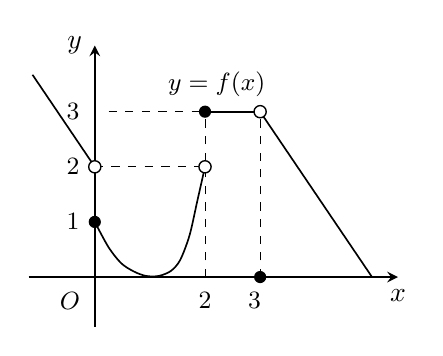
\begin{tikzpicture}[x=0.70cm, y=0.70cm, line width=0.5pt]
  \draw[->, >=stealth, line width=0.7pt] (-1.2,0) -- (5.5,0) node[below=1pt] {$x$};
  \draw[->, >=stealth, line width=0.7pt] (0,-0.9) -- (0,4.2) node[left=1pt] {$y$};
  \node[below=2pt, font=\small] at (-0.45,0) {$\pt{O}$};
  % 좌표 안내 파선(원문)
  \draw[dashed, line width=0.35pt] (0.25,3) -- (2,3);
  \draw[dashed, line width=0.35pt] (0,2) -- (2,2);
  \draw[dashed, line width=0.35pt] (2,0) -- (2,3);
  \draw[dashed, line width=0.35pt] (3,0) -- (3,3);
  % 그래프
  \draw[line width=0.6pt] (-1.13,3.67) -- (0,2);
  \draw[line width=0.6pt, smooth] plot coordinates {(0,1) (0.25,0.54) (0.48,0.25) (0.71,0.10) (0.93,0.02) (1.16,0.02) (1.38,0.11) (1.55,0.31) (1.72,0.76) (1.86,1.38) (2,2)};
  \draw[line width=0.6pt] (2,3) -- (3,3);
  \draw[line width=0.6pt] (3,3) -- (5.03,0);
  % 닫힌점
  \fill (0,1) circle (2.2pt);
  \fill (2,3) circle (2.2pt);
  \fill (3,0) circle (2.2pt);
  % 열린점
  \draw[fill=white, line width=0.5pt] (0,2) circle (2.2pt);
  \draw[fill=white, line width=0.5pt] (2,2) circle (2.2pt);
  \draw[fill=white, line width=0.5pt] (3,3) circle (2.2pt);
  % 눈금 라벨(원문 자리 그대로: y 눈금은 모두 축 왼쪽)
  \node[left=2pt, font=\small] at (0,3) {$3$};
  \node[left=2pt, font=\small] at (0,2) {$2$};
  \node[left=2pt, font=\small] at (0,1) {$1$};
  \node[below=2pt, font=\small] at (2,0) {$2$};
  \node[below=2pt, font=\small] at (2.9,0) {$3$};
  \node[right=1pt, font=\small] at (1.1,3.5) {$y=f(x)$};
\end{tikzpicture}
